\documentclass[a4paper, 11pt]{article}
\usepackage[python]{mypackage}
\usepackage{amsmath}
\usepackage{graphicx}
\usepackage{geometry}
\usepackage{listings}
\geometry{scale=0.8}
% \linespread{1.5}
\usepackage{hyperref}


\title{	
\normalfont \normalsize
\textsc{School of Data and Computer Science, Sun Yat-sen University} \\ [25pt] %textsc small capital letters
\rule{\textwidth}{0.5pt} \\[0.4cm] % Thin top horizontal rule
\huge  E09 Bayesian Network \\ % The assignment title
\rule{\textwidth}{2pt} \\[0.5cm] % Thick bottom horizontal rule
\author{17341015 Hongzheng Chen}
\date{\normalsize\today}
}

\begin{document}
\maketitle
\tableofcontents
\newpage

\section{Pomegranate Installation}
\textbf{Under Linux:}
\begin{enumerate}
\item Install \texttt{python} first (\textbf{python 2}, not python 3).
\item Run \texttt{sudo apt-get install python-pip} to install \texttt{pip}.
\item Run \texttt{sudo pip install pomegranate} to install \texttt{pomegranate}.
\end{enumerate}
\begin{figure}[h]
  \centering
  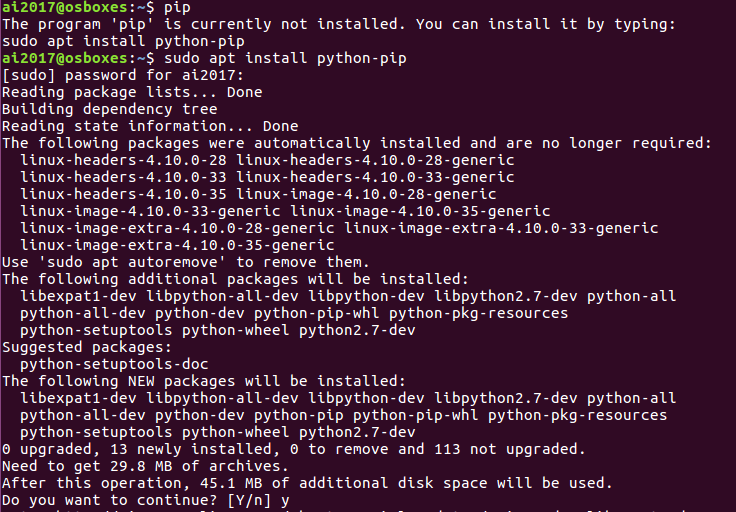
\includegraphics[width=7.5cm]{fig/install1}
  \qquad
  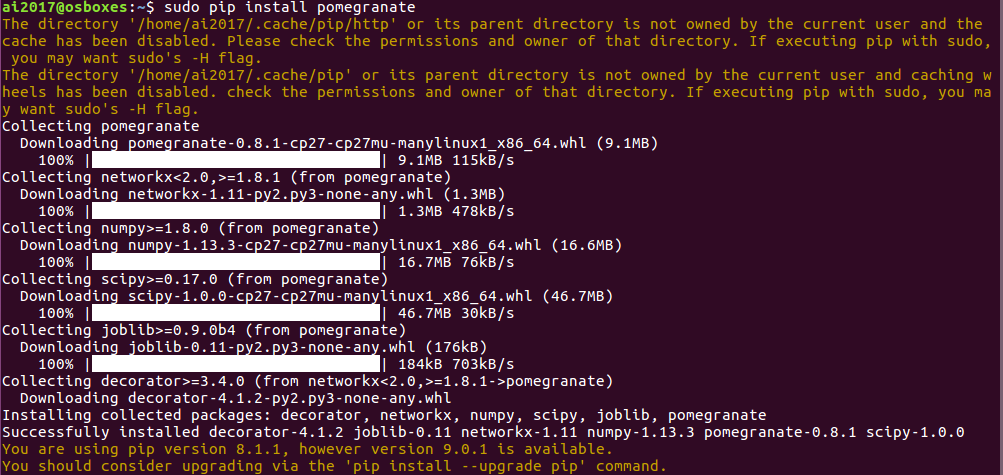
\includegraphics[width=8cm]{fig/install2}
\end{figure}
\textbf{Under Windows}

You can also run \texttt{pip install pomegranate} if you have installed \texttt{pip}. If you don't know how to install \texttt{pip}, please click \url{https://jingyan.baidu.com/article/e73e26c0d94e0524adb6a7ff.html}.

For more, please click the homepage of Pomegranate - \url{https://github.com/jmschrei/pomegranate} for help. 
\begin{figure}[h]

  
  \centering
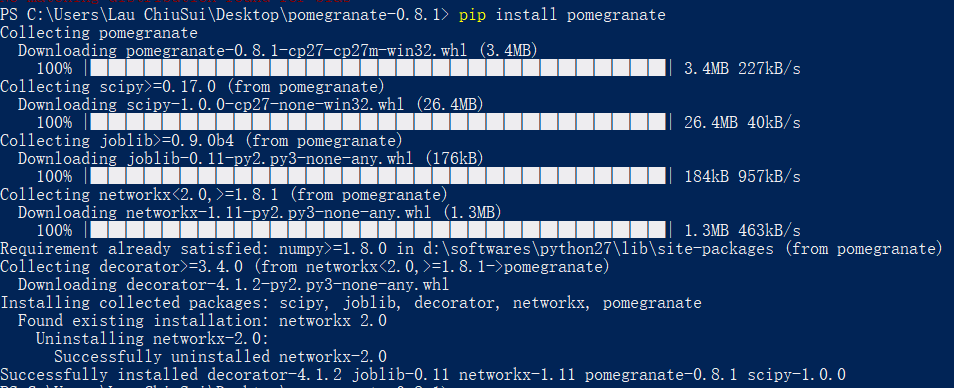
\includegraphics[width=16cm]{fig/po}
  
\end{figure}

\section{Building Bayesian Network}
\label{sec:build-bayes-netw}
Please refer to \texttt{Tutorial\_4\_Bayesian\_Networks.pdf}. I will explain it in class.

\section{Tasks}
\label{sec:tasks}

\subsection{Burglary}
\label{sec:burglary}
\begin{figure}[h]
  \centering

  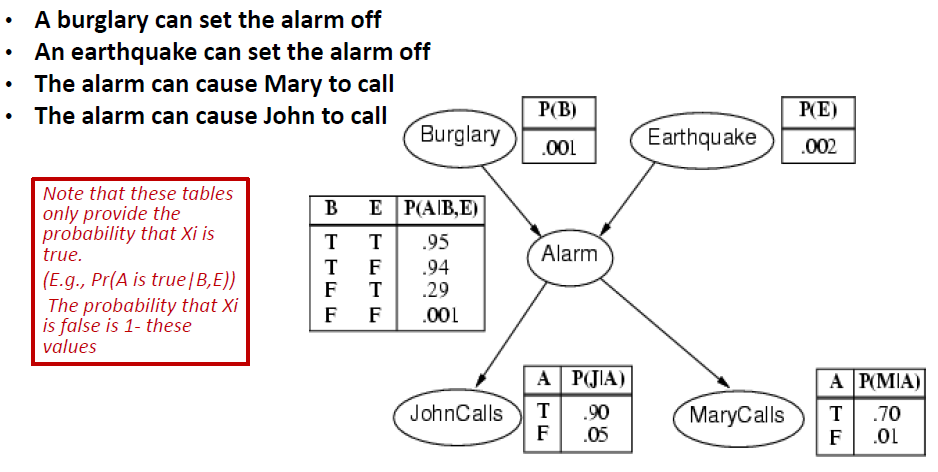
\includegraphics[width=14cm]{fig/burglary}
\end{figure}
Please code to calculate:
\begin{enumerate}
\item $P(A)$
\item $P(J\overline{M})$
\item $P(A | J\overline{M})$
\item $P(B | A)$
\item $P(B | J\overline{M})$
\item  $P(J\overline{M} | \overline{B})$
\end{enumerate}
\begin{figure}[ht]
\centering
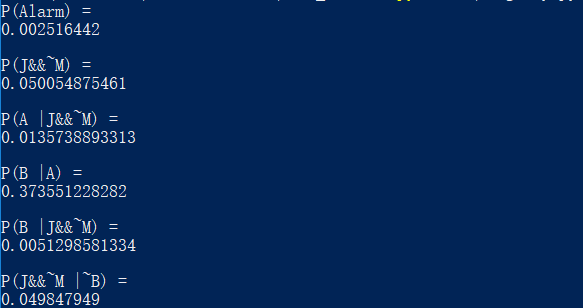
\includegraphics[width=12cm]{fig/burglar_result}
\end{figure}
\subsection{Diagnosing}
\label{sec:bayesian-networks}
\textbf{Variables and their domais}
\begin{lstlisting}
(1)PatientAge:['0-30','31-65','65+']
(2)CTScanResult:['Ischemic Stroke','Hemmorraghic Stroke']
(3)MRIScanResult: ['Ischemic Stroke','Hemmorraghic Stroke']
(4)StrokeType: ['Ischemic Stroke','Hemmorraghic Stroke', 'Stroke Mimic']
(5)Anticoagulants: ['Used','Not used']
(6)Mortality:['True', 'False']
(7)Disability: ['Negligible', 'Moderate', 'Severe']
\end{lstlisting}
\textbf{CPTs}

\textbf{Note:} [CTScanResult, MRIScanResult,StrokeType] means:

P(StrokeType='...' $|$ CTScanResult='...' $\land$  MRIScanResult='...') 
\begin{lstlisting}
(1)
[PatientAge]

['0-30', 0.10],
['31-65', 0.30],
['65+', 0.60]

(2)
[CTScanResult]

['Ischemic Stroke',0.7],
[ 'Hemmorraghic Stroke',0.3]

(3)
[MRIScanResult]

['Ischemic Stroke',0.7],
[ 'Hemmorraghic Stroke',0.3]

(4)
[Anticoagulants]

['Used',0.5],
['Not used',0.5]

(5)
[CTScanResult, MRIScanResult,StrokeType]

['Ischemic Stroke','Ischemic Stroke','Ischemic Stroke',0.8],
['Ischemic Stroke','Hemmorraghic Stroke','Ischemic Stroke',0.5],  
[ 'Hemmorraghic Stroke','Ischemic Stroke','Ischemic Stroke',0.5],
[ 'Hemmorraghic Stroke','Hemmorraghic Stroke','Ischemic Stroke',0], 

['Ischemic Stroke','Ischemic Stroke','Hemmorraghic Stroke',0],
['Ischemic Stroke','Hemmorraghic Stroke','Hemmorraghic Stroke',0.4], 
[ 'Hemmorraghic Stroke','Ischemic Stroke','Hemmorraghic Stroke',0.4],
[ 'Hemmorraghic Stroke','Hemmorraghic Stroke','Hemmorraghic Stroke',0.9],

['Ischemic Stroke','Ischemic Stroke','Stroke Mimic',0.2],
['Ischemic Stroke','Hemmorraghic Stroke','Stroke Mimic',0.1],    
[ 'Hemmorraghic Stroke','Ischemic Stroke','Stroke Mimic',0.1],
[ 'Hemmorraghic Stroke','Hemmorraghic Stroke','Stroke Mimic',0.1],

(6) 
[StrokeType, Anticoagulants, Mortality]

['Ischemic Stroke', 'Used', 'False',0.28],
['Hemmorraghic Stroke', 'Used', 'False',0.99],
['Stroke Mimic', 'Used', 'False',0.1],
['Ischemic Stroke','Not used', 'False',0.56],
['Hemmorraghic Stroke', 'Not used', 'False',0.58],
['Stroke Mimic', 'Not used', 'False',0.05],

['Ischemic Stroke',  'Used' ,'True',0.72],
['Hemmorraghic Stroke', 'Used', 'True',0.01],
['Stroke Mimic', 'Used', 'True',0.9],
['Ischemic Stroke',  'Not used' ,'True',0.44],
['Hemmorraghic Stroke', 'Not used', 'True',0.42 ],
['Stroke Mimic', 'Not used', 'True',0.95]

(7)
[StrokeType, PatientAge, Disability]

['Ischemic Stroke',   '0-30','Negligible', 0.80],
['Hemmorraghic Stroke', '0-30','Negligible', 0.70],
['Stroke Mimic',        '0-30', 'Negligible',0.9],
['Ischemic Stroke',     '31-65','Negligible', 0.60],
['Hemmorraghic Stroke', '31-65','Negligible', 0.50],
['Stroke Mimic',        '31-65', 'Negligible',0.4],
['Ischemic Stroke',     '65+'  , 'Negligible',0.30],
['Hemmorraghic Stroke', '65+'  , 'Negligible',0.20],
['Stroke Mimic',        '65+'  , 'Negligible',0.1],

['Ischemic Stroke',     '0-30' ,'Moderate',0.1],
['Hemmorraghic Stroke', '0-30' ,'Moderate',0.2],
['Stroke Mimic',        '0-30' ,'Moderate',0.05],
['Ischemic Stroke',     '31-65','Moderate',0.3],
['Hemmorraghic Stroke', '31-65','Moderate',0.4],
['Stroke Mimic',        '31-65','Moderate',0.3],
['Ischemic Stroke',     '65+'  ,'Moderate',0.4],
['Hemmorraghic Stroke', '65+'  ,'Moderate',0.2],
['Stroke Mimic',        '65+'  ,'Moderate',0.1],

['Ischemic Stroke',     '0-30' ,'Severe',0.1],
['Hemmorraghic Stroke', '0-30' ,'Severe',0.1],
['Stroke Mimic',        '0-30' ,'Severe',0.05],
['Ischemic Stroke',     '31-65','Severe',0.1],
['Hemmorraghic Stroke', '31-65','Severe',0.1],
['Stroke Mimic',        '31-65','Severe',0.3],
['Ischemic Stroke',     '65+'  ,'Severe',0.3],
['Hemmorraghic Stroke', '65+'  ,'Severe',0.6],
['Stroke Mimic',        '65+'  ,'Severe',0.8]
\end{lstlisting}
\textbf{Calculation}

Please code to calculate the following probability value:

p1 = P(Mortality='True' $|$ PatientAge='31-65' $\land$ CTScanResult='Ischemic Stroke')

p2 = P(Disability='Moderate' $|$ PatientAge='65+' $\land$  MRIScanResult='Hemmorraghic Stroke')

p3 = P(StrokeType='Stroke Mimic' $|$ PatientAge='65+' $\land$ CTScanResult='Hemmorraghic Stroke' $\land$ MRIScanResult='Ischemic Stroke')

p4 = P(Anticoagulants='Not used' $|$ PatientAge='0-30')

\begin{figure}[ht]
\centering
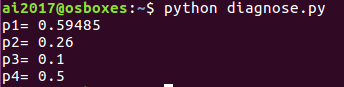
\includegraphics[width=12cm]{fig/diagnose_result}
\end{figure}

Please solve the 2 tasks and hand in a file named \textsf{E09\_YourNumber.pdf}, and send it to \textsf{ai\_201901@foxmail.com}


\section{Codes and Results}
\textcolor{red}{The codes use Python 3!}
\begin{figure}[H]
\centering
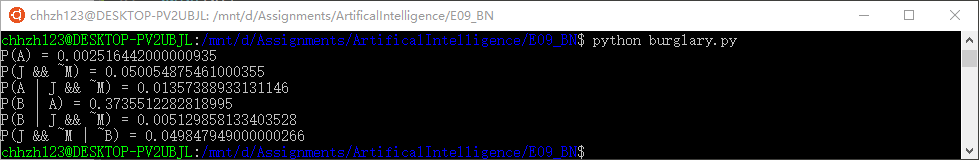
\includegraphics[width=\linewidth]{fig/result1.png}
\end{figure}
\begin{lstlisting}[title=burglary.py]
from pomegranate import *

burglary = DiscreteDistribution( {'T':0.001, 'F':0.999} )
earthquake = DiscreteDistribution( {'T':0.002, 'F':0.998} )
alarm = ConditionalProbabilityTable(
	[['T','T','T',0.95],
	 ['T','F','T',0.94],
	 ['F','T','T',0.29],
	 ['F','F','T',0.001],
	 ['T','T','F',0.05],
	 ['T','F','F',0.06],
	 ['F','T','F',0.71],
	 ['F','F','F',0.999]], [burglary, earthquake])
johncalls = ConditionalProbabilityTable(
	[['T','T',0.90],
	 ['F','T',0.05],
	 ['T','F',0.10],
	 ['F','F',0.95]], [alarm])
marycalls = ConditionalProbabilityTable(
	[['T','T',0.70],
	 ['F','T',0.01],
	 ['T','F',0.30],
	 ['F','F',0.99]], [alarm])

s1 = State(burglary, name="burglary")
s2 = State(earthquake, name="earthquake")
s3 = State(alarm, name="alarm")
s4 = State(johncalls, name="johncalls")
s5 = State(marycalls, name="marycalls")

model = BayesianNetwork("Burglary")

model.add_states(s1,s2,s3,s4,s5)

model.add_transition(s1,s3)
model.add_transition(s2,s3)
model.add_transition(s3,s4)
model.add_transition(s3,s5)
model.bake()

marginals = model.predict_proba({})
# P(A)
print("P(A) = {}".format(marginals[2].parameters[0]["T"]))
# P(J&&~M) = P(J|~M)P(~M)
j_nm = model.predict_proba({'marycalls':'F'})[3].parameters[0]["T"] * marginals[4].parameters[0]["F"]
print("P(J && ~M) = {}".format(j_nm))
# P(A|J&&~M)
print("P(A | J && ~M) = {}".format(model.predict_proba({'johncalls':'T','marycalls':'F'})[2].parameters[0]["T"]))
# P(B|A)
print("P(B | A) = {}".format(model.predict_proba({'alarm':'T'})[0].parameters[0]["T"]))
# P(B|J&&~M)
b_c_j_nm = model.predict_proba({'johncalls':'T','marycalls':'F'})[0].parameters[0]["T"]
print("P(B | J && ~M) = {}".format(b_c_j_nm))
# P(J&&~M|~B) = P(~B && J && ~M) / P(~B)
#             = P(~B | J && ~M) P(J && ~M) / P(~B)
#             = (1- P(B | J && ~M)) P(J && ~M) / P(~B)
print("P(J && ~M | ~B) = {}".format((1-b_c_j_nm) * j_nm / marginals[0].parameters[0]["F"]))
\end{lstlisting}

\begin{figure}[H]
\centering
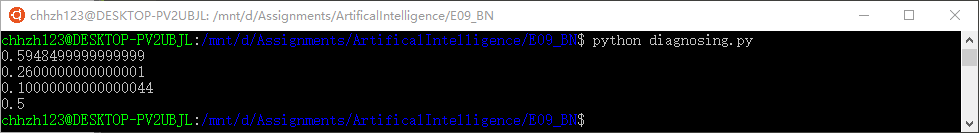
\includegraphics[width=\linewidth]{fig/result2.png}
\end{figure}
\begin{lstlisting}[title=diagnosing.py]
from pomegranate import *

PatientAge = DiscreteDistribution({'0-30':0.10, '31-65':0.30, '65+':0.60})
CTScanResult = DiscreteDistribution({'Ischemic Stroke':0.7, 'Hemmorraghic Stroke':0.3})
MRIScanResult = DiscreteDistribution({'Ischemic Stroke':0.7, 'Hemmorraghic Stroke':0.3})
Anticoagulants = DiscreteDistribution({'Used':0.5 ,'Not used':0.5})

StrokeType = ConditionalProbabilityTable(
	[['Ischemic Stroke','Ischemic Stroke','Ischemic Stroke',0.8],
	 ['Ischemic Stroke','Hemmorraghic Stroke','Ischemic Stroke',0.5],
	 ['Hemmorraghic Stroke','Ischemic Stroke','Ischemic Stroke',0.5],
	 ['Hemmorraghic Stroke','Hemmorraghic Stroke','Ischemic Stroke',0],
	 ['Ischemic Stroke','Ischemic Stroke','Hemmorraghic Stroke',0],
	 ['Ischemic Stroke','Hemmorraghic Stroke','Hemmorraghic Stroke',0.4],
	 ['Hemmorraghic Stroke','Ischemic Stroke','Hemmorraghic Stroke',0.4],
	 ['Hemmorraghic Stroke','Hemmorraghic Stroke','Hemmorraghic Stroke',0.9],
	 ['Ischemic Stroke','Ischemic Stroke','Stroke Mimic',0.2],
	 ['Ischemic Stroke','Hemmorraghic Stroke','Stroke Mimic',0.1],
	 ['Hemmorraghic Stroke','Ischemic Stroke','Stroke Mimic',0.1],
	 ['Hemmorraghic Stroke','Hemmorraghic Stroke','Stroke Mimic',0.1]],[CTScanResult,MRIScanResult])
Mortality = ConditionalProbabilityTable(
	[['Ischemic Stroke','Used','False',0.28],
	 ['Hemmorraghic Stroke','Used','False',0.99],
	 ['Stroke Mimic','Used','False',0.1],
	 ['Ischemic Stroke','Not used','False',0.56],
	 ['Hemmorraghic Stroke','Not used','False',0.58],
	 ['Stroke Mimic','Not used','False',0.05],
	 ['Ischemic Stroke','Used','True',0.72],
	 ['Hemmorraghic Stroke','Used','True',0.01],
	 ['Stroke Mimic','Used','True',0.9],
	 ['Ischemic Stroke','Not used','True',0.44],
	 ['Hemmorraghic Stroke','Not used','True',0.42],
	 ['Stroke Mimic','Not used','True',0.95]],[StrokeType, Anticoagulants])
Disability = ConditionalProbabilityTable(
	[['Ischemic Stroke','0-30','Negligible',0.80],
	['Hemmorraghic Stroke','0-30','Negligible',0.70],
	['Stroke Mimic','0-30','Negligible',0.9],
	['Ischemic Stroke','31-65','Negligible',0.60],
	['Hemmorraghic Stroke','31-65','Negligible',0.50],
	['Stroke Mimic','31-65','Negligible',0.4],
	['Ischemic Stroke','65+','Negligible',0.30],
	['Hemmorraghic Stroke','65+','Negligible',0.20],
	['Stroke Mimic','65+','Negligible',0.1],
	['Ischemic Stroke','0-30','Moderate',0.1],
	['Hemmorraghic Stroke','0-30','Moderate',0.2],
	['Stroke Mimic','0-30','Moderate',0.05],
	['Ischemic Stroke','31-65','Moderate',0.3],
	['Hemmorraghic Stroke','31-65','Moderate',0.4],
	['Stroke Mimic','31-65','Moderate',0.3],
	['Ischemic Stroke','65+','Moderate',0.4],
	['Hemmorraghic Stroke','65+','Moderate',0.2],
	['Stroke Mimic','65+','Moderate',0.1],
	['Ischemic Stroke','0-30','Severe',0.1],
	['Hemmorraghic Stroke','0-30','Severe',0.1],
	['Stroke Mimic','0-30','Severe',0.05],
	['Ischemic Stroke','31-65','Severe',0.1],
	['Hemmorraghic Stroke','31-65','Severe',0.1],
	['Stroke Mimic','31-65','Severe',0.3],
	['Ischemic Stroke','65+','Severe',0.3],
	['Hemmorraghic Stroke','65+','Severe',0.6],
	['Stroke Mimic','65+','Severe',0.8]],[StrokeType,PatientAge])

s1 = State(PatientAge, name="PatientAge")
s2 = State(CTScanResult, name="CTScanResult")
s3 = State(MRIScanResult, name="MRIScanResult")
s4 = State(StrokeType, name="StrokeType")
s5 = State(Anticoagulants, name="Anticoagulants")
s6 = State(Mortality, name="Mortality")
s7 = State(Disability, name="Disability")

model = BayesianNetwork("Diagnosing")

model.add_states(s1,s2,s3,s4,s5,s6,s7)

model.add_transition(s2,s4)
model.add_transition(s3,s4)

model.add_transition(s4,s6)
model.add_transition(s5,s6)

model.add_transition(s1,s7)
model.add_transition(s4,s7)

model.bake()

marginals = model.predict_proba({})

p1 = model.predict_proba({'PatientAge':'31-65','CTScanResult':'Ischemic Stroke'})[5].parameters[0]["True"]
p2 = model.predict_proba({'PatientAge':'65+','MRIScanResult':'Hemmorraghic Stroke'})[6].parameters[0]["Moderate"]
p3 = model.predict_proba({'PatientAge':'65+','CTScanResult':'Hemmorraghic Stroke','MRIScanResult':'Ischemic Stroke'})[3].parameters[0]["Stroke Mimic"]
p4 = model.predict_proba({'PatientAge':'0-30'})[4].parameters[0]["Not used"]
print(p1)
print(p2)
print(p3)
print(p4)
\end{lstlisting}

%\clearpage
%\bibliography{E:/Papers/LiuLab}
%\bibliographystyle{apalike}
\end{document}